% Created 2021-01-24 Sun 22:50
% Intended LaTeX compiler: pdflatex
\documentclass[11pt]{article}
\usepackage[utf8]{inputenc}
\usepackage[T1]{fontenc}
\usepackage{graphicx}
\usepackage{grffile}
\usepackage{longtable}
\usepackage{wrapfig}
\usepackage{rotating}
\usepackage[normalem]{ulem}
\usepackage{amsmath}
\usepackage{textcomp}
\usepackage{amssymb}
\usepackage{capt-of}
\usepackage{hyperref}
\usepackage{minted}
\hypersetup{colorlinks=true, linkcolor=black, filecolor=red, urlcolor=blue}
\usepackage[turkish]{babel}
\author{Eren Hatırnaz}
\date{3 Kasım 2019}
\title{Yazılım Gündemi - 16\\\medskip
\large 28 Ekim - 3 Kasım 2019}
\hypersetup{
 pdfauthor={Eren Hatırnaz},
 pdftitle={Yazılım Gündemi - 16},
 pdfkeywords={},
 pdfsubject={},
 pdfcreator={Emacs 27.1 (Org mode 9.3)},
 pdflang={Turkish}}
\begin{document}

\maketitle
\tableofcontents \clearpage\shorthandoff{=}

\begin{center}
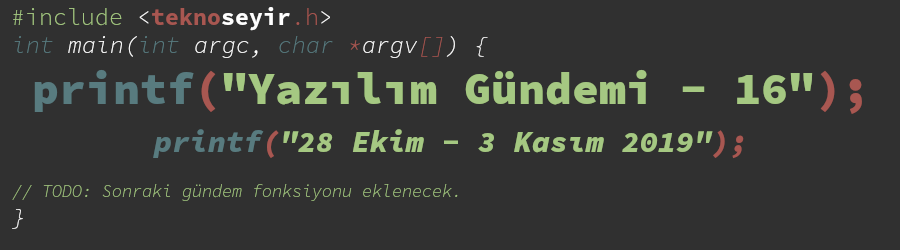
\includegraphics[width=.9\linewidth]{gorseller/yazilim-gundemi-banner.png}
\end{center}

\begin{center}
\href{../15/yazilim-gundemi-15.pdf}{< Önceki Gündem} | \textbf{28 Ekim - 3 Kasım 2019} | \href{../17/yazilim-gundemi-17.pdf}{Sonraki Gündem >}

\href{https://teknoseyir.com/blog/yazilim-gundemi-16-28-ekim-3-kasim-2019}{TeknoSeyir'de Oku}
\end{center}

\section{Notepad++ 7.8.1 sürümünü \href{https://notepad-plus-plus.org/news/v781-free-uyghur-edition/}{"Free Uyghur" ismiyle çıkardı}}
\label{sec:org91d163f}
\begin{center}

\includegraphics[height=2cm]{gorseller/notepadpp-free-uyghur.png}
\end{center}

Notepad++ her ne kadar doğrudan bir programlama aracı olmasa da hızlı
çalışmasından dolayı Windows ortamında tercih edilebilen bir metin editörü.
Geliştiricisi Don Ho, bu hafta duyurduğu 7.8.1 sürümünün ismini, Çin'de Uygur
Türk'lerine uygulanan 'yeniden eğitim kampları'na dikkat çekmek için "Free
Uyghur" ("Uygurlara özgürlük") koydu.

29 Ekim tarihinde yayınladığı blog yazısında Çin devletinin yaptığı insan
haklarına aykırı şeylerden bahsetmekle kalmamış, oradaki insanlara nasıl yardım
edilebileceği ilgili de bilgi vermiş. Fakat benim özellikle dikkat çekmek
istediğim kısım yazısının son paragrafı, Türkçe'ye çevirecek olursak:

\begin{quote}
İnsanlar bana tekrardan "programlamayı ya da işi siyaset ile karıştırma"
diyecekler. Bunu yapmak kesinlikle Notepad++'ın popülaritesini etkiler: Siyaset
hakkında konuşmak, yazılım ve ticari şirketlerin genellikle kaçınmaya çalıştığı
şeydir. Problem şudur ki: \uline{Eğer biz siyaset ile uğraşmazsak, siyaset bizimle
uğraşır}. İnsanlar ezildiğinde hareket etmemeyi seçebilirsiniz, ama ezilme
sıramız geldiğinde, çok geç olacak ve bizim için kimse olmayacak. \uline{Harekete
geçmeniz için Uygur ya da Müslüman olmanız gerekmiyor},
\uline{sadece insan olmak ve bazı insanlarla empati kurabilmek yeterli}.
\end{quote}

Çok iyi çevirememiş olabilirim (yanlış çevirdiğimi düşündüğünüz yerleri
yorumlar bölümünde belirtebilirsiniz) fakat vermek istediği mesajı anlamak için
yeterli olduğunu düşünüyorum. "Biz siyasetle uğraşmazsak, siyaset bizimle
uğraşır" sözünü ben en iyi 2016 yılında anlamıştım. Berat Albayrak'ın maili
hackleyen RedHack grubu, mailleri GitHub'a yükleyince \href{https://teknoseyir.com/durum/1155906}{GitHub 1 gün boyun
boyunca yasaklı kaldı}. Görüyorsunuz, siz ne kadar siyaset ile ilgilenmemeye
çalışsanız da bir şekilde geliyor buluyor sizi. İster programlama, ister bilim
yapıyor olun. İşte bu yüzden "açık kaynak" yerine "özgür yazılım" hareketini
destekliyorum. Don Ho'nun blog yazısındaki bu son paragrafı gerçekten çok
önemli. Bunları hiç çekinmeden dile getirmesinden dolayı geliştirici arkadaşı
kutlamak gerek. Böyle insanların var olduğunu bilmek dünyaya dair umutlarımı
bir nebze olsun yeşertiyor. Bu konu hakkında siz ne düşünüyorsunuz? Sizce
yazılım ve siyaset birbirinden tamamen ayrı konular mı yoksa sürekli olmasa da
birbirlerini etkileyen şeyler mi? Yazılımcılar olarak ne kadar ilgilenmeliyiz
bu konularla? Yorumlar kısmında konuşalım.

\begin{center}
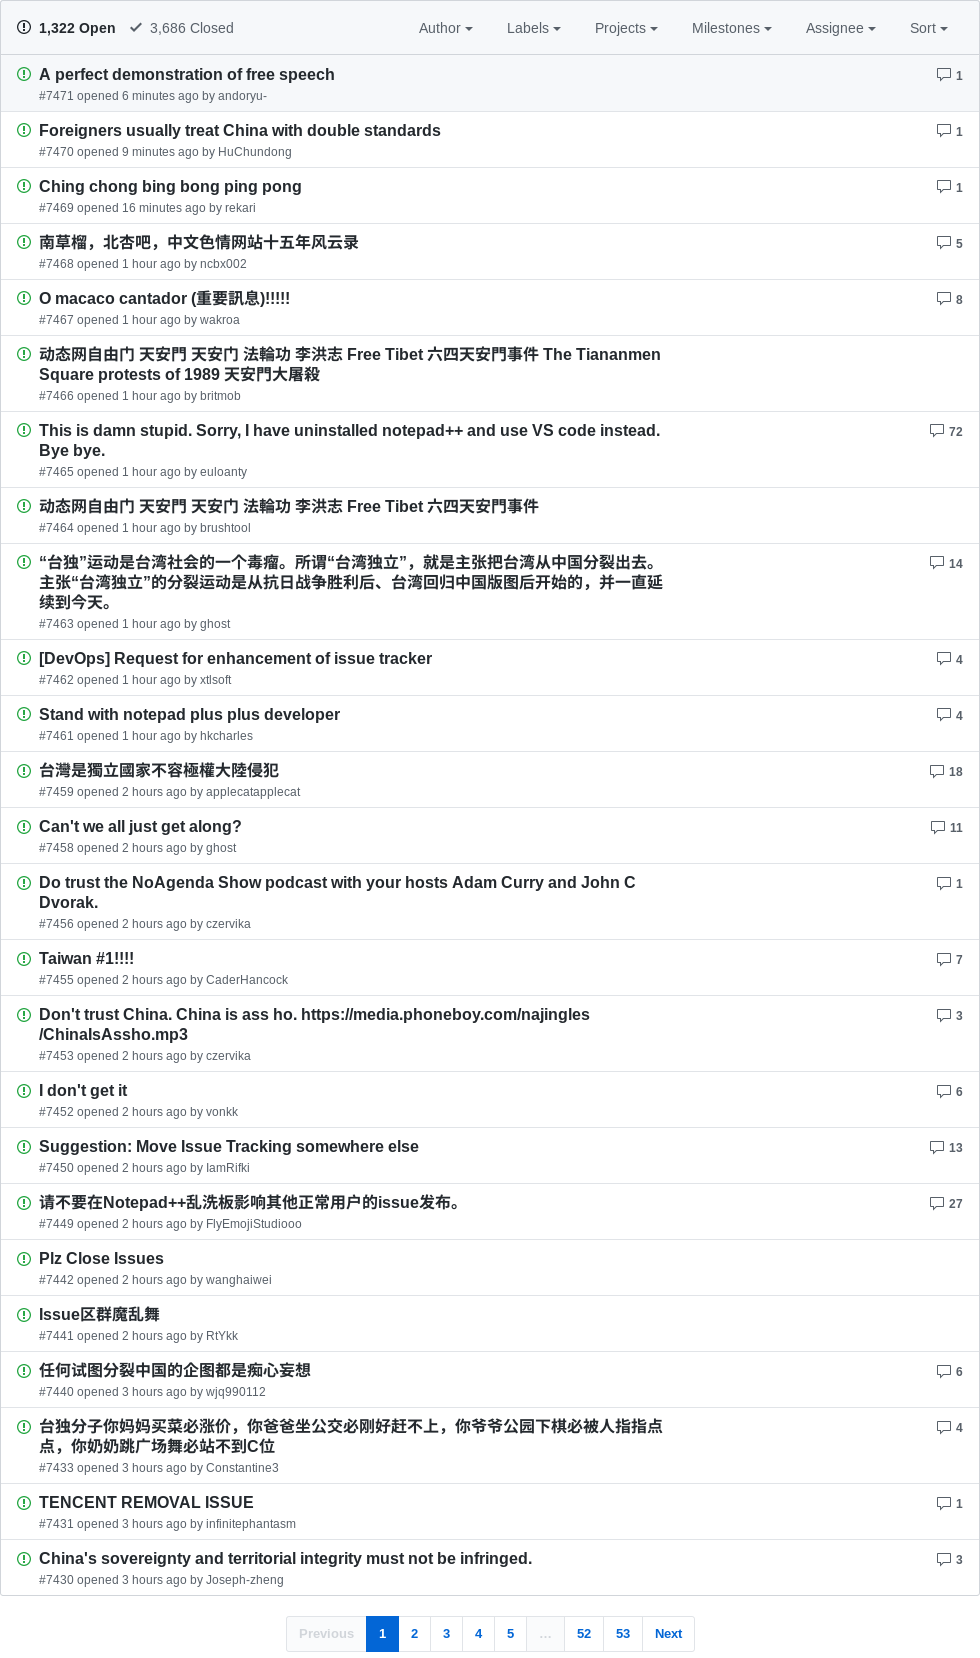
\includegraphics[height=10cm]{gorseller/notepadpp-issues-spam.png}
\end{center}

Bir nebze olsun umut yeşerten insanlardan ziyade maalesef aynı dünyada
olduğumuzdan dolayı utanç duyacağımız insanlar da var. Bu blog yazısının
yayınladığı saatten sonra Notepad++ projesinin \href{https://github.com/notepad-plus-plus/notepad-plus-plus/issues}{GitHub sayfasının Issues bölümü}
birçok Çinli vatandaş tarafından \href{https://www.zdnet.com/article/chinese-users-attack-notepad-app-after-free-uyghur-release/}{spam yağmuruna tutuldu}. "Çin'de öyle şeyler
yapılmıyor" diyenden tut da, bayağı küfürlü mesajlar yazanlara kadar yüzlerce
hatta binlerce spam issue sayfası açıldı. Ne söylenebilir ki bu insanlar
için\ldots{} (aslında söylenebilecek bazı şeyler var da burası yeri değil)
\section{İspanya'nın isteği üzerine GitHub protestocuların kullandığı \href{https://www.vice.com/en\_ca/article/9kevn7/spain-and-github-are-blocking-an-app-that-helped-protesters-organize}{uygulamanın deposunu kaldırdı}}
\label{sec:org622d0b0}
İspanya'nın Barcelona kentinde yaklaşık bir aydır devam eden protestolar var.
Bu protestoların sebebi ayrıkçı Katalan liderlerinin ve Katalonya'nın
bağımsızlığını destekleyenlerin tutuklanması. Bu haberin yazılım gündemine
girmesinin sebebi ise, kendilerine Tsunami Democrátic diyen aktivist bir grubun
protestocuların kullanması için geliştirdiği bir mobil uygulamanın GitHub'dan,
hükumet istediği doğrultusunda silinmesi. Bunu da GitHub'ın, hükumetlerden
kendisine gelen kapatma isteklerini paylaştığı \href{https://github.com/github/gov-takedowns}{deposundan öğreniyoruz}.
Görüyoruz ki, Rusya ve Çin ülkelerinin arasına bir de İspanya eklenmiş.

Tsunami Democrátic grubunun github üzerinde \href{https://tsunamidemocratic.github.io/}{barındırdığı web sitesi} yayında
kalmaya devam ediyor (İspanya'da engellenmiş, biz görebiliyoruz) fakat
uygulamanın APK dosyasının olduğu depo, GitHub tarafından silinmiş. İlgili
aktivist grup da bu sefer kendilerine başka bir yol bulmuşlar: bir \href{https://t.me/apptsunamidemocratic}{telegram
kanalı} hazırlamışlar ve APK dosyasını oradan dağıtıyorlar.
\section{Android 11 sürümünde kablosuz bağlantı üzerinden \href{https://www.xda-developers.com/android-11-native-wireless-adb/}{ADB desteği gelebilir}}
\label{sec:org6f7f5cb}
\href{https://www.xda-developers.com/install-adb-windows-macos-linux/}{Android Debug Bridge (ADB)} isminden de anlaşılacağı üzere, Android uygulama
geliştirirken hata ayıklama ve diğer birçok farklı işlem için
kullanabileceğiniz Android geliştiricinin takım çantasında mutlaka olması
gereken bir araç. Android geliştirme ile çok az deneyimim olsa da \href{https://www.xda-developers.com/install-adb-windows-macos-linux/}{Android Debug
Bridge (ADB)} aracının Android geliştiriciler için ne kadar önemli olduğunu
biliyorum. Bu özellik henüz sadece USB bağlantı üzerinden kullanılabilir fakat
bazı geliştiriciler hem kablo ile uğraşmamak için hem de birden fazla cihazda
geliştirme yaparken kablosuz olarak da bu özelliği kullanmak istiyor. ADB aracı
buna izin veriyor fakat yine ilk bağlantı için USB'yi bağlayıp sonra kablosuz
olarak devam etmek ve birden fazla cihazla çalışıyorsanız da her cihaza sabit
bir IP adresi vermek gerekiyor-ki router kapatıp açılınca lokal IP adresler de
değişmesin. Üstelik bu yöntem hiç de güvenli değil, çünkü bağlantı TCP/IP
protokolü üzerinden şifresiz bir şekilde düz metin olarak kuruluyor.
Dolayısıyla güvenmediğiniz ağlarda kullanamıyorsunuz.

Bu hafta xda-developers sitesindeki bir üyenin fark etmesiyle anlaşıldı ki bir
google çalışanının bu özellikle ilgili commit'ler yapmış. İlgili commit'ler şu
şekilde:
\begin{itemize}
\item \href{https://android-review.googlesource.com/c/platform/system/core/+/1148015}{1148015: Add wifi service for adb.}
\item \href{https://android-review.googlesource.com/c/platform/system/core/+/1148676}{1148676: WIP implement secure pairing for ADB Wireless}
\end{itemize}
Commit mesajlarından ve içeriklerinden anlayabileceğiniz üzere Google'da bu
yönde bir çalışma var. Androd'in Geliştirici Ayarları kısmına "Wireless
debugging" anahtarı eklenmiş ve üstelik güvenli olabilmesi için de kablosuz
bağlantı kurulurken QR kod ya da 6 haneli bir kod ile eşleşme gerekli olacak
gibi gözüküyor. Fakat Android geliştirici arkadaşların hemen heyecanlanmasını
tavsiye etmiyorum. Çünkü değişiklikler henüz merge edilmemiş gözüküyor.
xda-developers sitesindeki geliştiricilerin de Android 11'de bu özelliğin
kullanıma sunulmasını umuyorlar fakat bekleyip görmek gerek. Umarım Android
geliştirici arkadaşların işlerini kolaylaştıracak bu özellik yakın zamanda
gelir.
\section{Python, 3.9 sürümünden sonra \href{https://lwn.net/Articles/803679/}{yıllık sürüm döngüsüne adapte olacak}}
\label{sec:org51fcdfd}
30 Ekim tarihinde yönetim kurulu üyesi Brett Cannon'un Python geliştiricileri
e-posta grubuna gönderdiği maile göre daha önce Łukasz Langa tarafından
önerilen \href{https://www.python.org/dev/peps/pep-0602/}{PEP 602 - Annual Release Cycle for Python} önerisi kabul edildi. İlgili
önerinin sayfasında durumu henüz "Draft" (Taslak) olarak gözükse de gönderilen
mailde kısa süre içinde sayfanın güncelleneceğini belirtilmiş. Daha önce de 18
aylık sürüm döngüsündeydiler.

Bu yeni döngüye göre artık herhangi bir Python 3.X.0 sürümü bu şekilde
hazırlanacak:
\begin{enumerate}
\item Python 3.X.0'ın geliştirilmesine, Python 3.(X-1).0 Beta 1 sürümü
yayınlandığında başlanacak ve 5 ay boyunca bu süreç versiyonlama olmadan
Pre-Alpha adı altında devam edecek.
\item Sonrasında 7 aylık yeni özelliklerin Alpha sürümler olarak duyurulacağı
periyot başlayacak. Her ay bir Alpha sürümü olacak şekilde toplamda 7
Alpha sürümü çıkacak.
\item Sonrasında 4 aylık herhangi bir yeni özellik içermeyen Beta süreci
başlayacak ve bu süreç boyunca kullanıcılardan gelen hata raporları
incelenip onlar giderilecek.
\item Sonrasında 1 aylık Release Candidate süreci başlayacak ve ayın bitiminde
Python 3.X.0 final sürümü duyurulmuş olacak.
\end{enumerate}
Yani herhangi bir Python 3.X.0 sürümü 17 ay içerisinde geliştirilecek ve
sürümler halinde önümüze sunulacak. Yalnız gönderilen mailde Beta ve RC
süreçleri ile ilgili birkaç değişiklik olabilir deniyor. Final sürümünden
sonraki destek süreci de bu şekilde olacak:
\begin{enumerate}
\item Final sürümden sonraki 18 ay (1.5 yıl) boyunca sürüm tam destek alacak.
\item Sonraki 42 ay (3.5 yıl) boyunca ise sadece güvenlik güncelleştirmeleri
alacak.
\end{enumerate}

\begin{figure}[htbp]
\centering
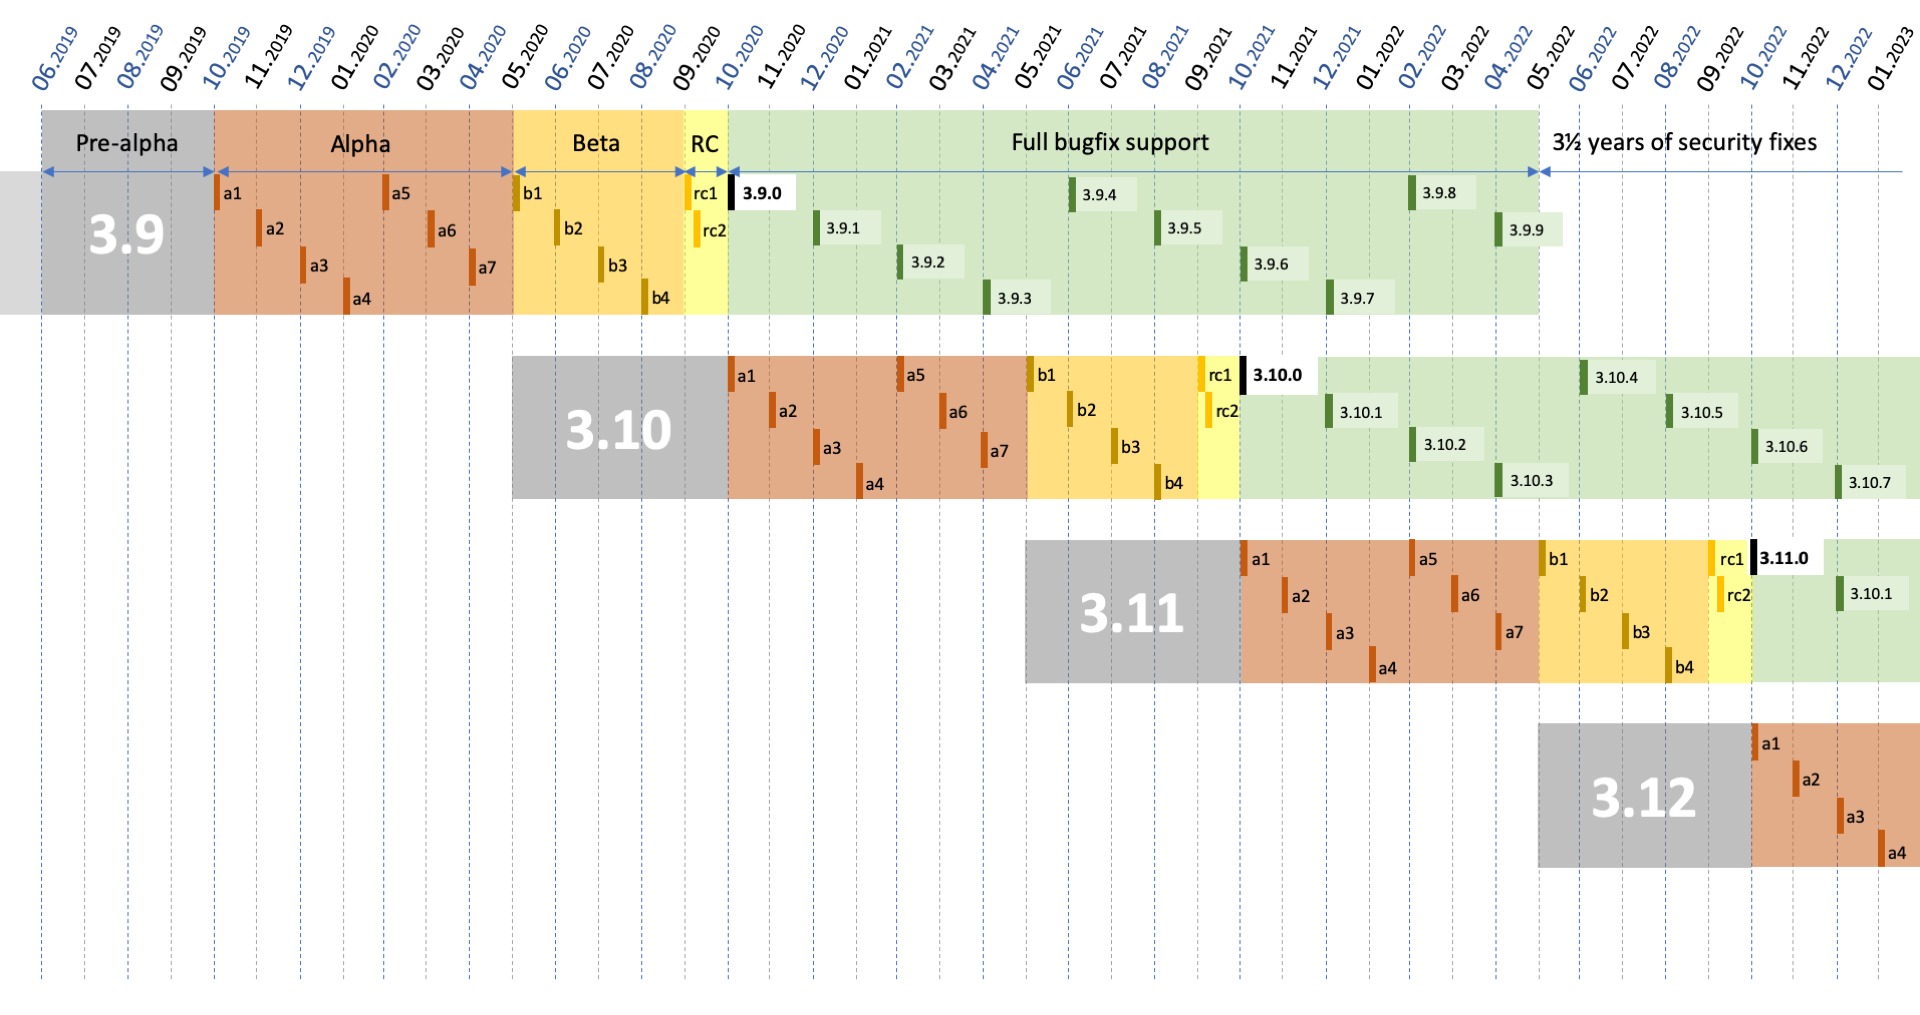
\includegraphics[width=.9\linewidth]{gorseller/python-omur.png}
\caption{Herhangi bir Python 3.X.0 sürümünün yaşam döngüsü böyle olacak.}
\end{figure}

Bu takvim güncellemesinin nedenlerinin bir kaçı ise şu şekilde:
\begin{itemize}
\item Sürümleri daha küçük yapmak.
\item Yeni özellikleri ve hata gidermelerini daha kısa sürede kullanıcıyla
buluşturmak.
\item Kullanıcılara daha iyi bir sürüm güncelleştirme yolu sunmak.
\item Daha tahmin edilebilir bir güncelleme takvimi sunmak.
\item Diğer nedenler için ilgili PEP sayfasındaki \href{https://www.python.org/dev/peps/pep-0602/\#id12}{Rationale and Goals} başlığına
bakabilirsiniz.
\end{itemize}

Projelerinde sıkça Python kullanan biriyseniz ya da Python üzerinden ürünler ya
da hizmetler veren bir şirkette çalışıyorsanız gözünüz mutlaka bu PEP
sayfasında olsun. İlgili değişikliklerden sonra bu PEP onaylanacak.

Ayrıca Python'ın yaratıcısı Guido van Rossum da en son çalıştığı Dropbox
şirketinden ayrılmış ve \href{https://www.zdnet.com/article/python-programming-language-creator-retires-saying-its-been-an-amazing-ride/}{emekliliğe ayrıldığını duyurmuş}. Kendisine bundan
sonraki yaşamında huzur ve mutluluklar dileriz.
\section{Cloudflare Rust ile yazılmış \href{https://blog.cloudflare.com/announcing-cfnts/}{NTS implementasyonunu duyurdu}: \href{https://github.com/cloudflare/cfnts}{cfnts}}
\label{sec:orgfeef861}
Geçtiğimiz aylarda Cloudflare'in, insanların pek fazla ilgilenmediği bir konu
olan \href{https://blog.cloudflare.com/secure-time/}{tarih/saat sunucularının güvenliği} hakkında yeni bir servis açtığını
\href{https://teknoseyir.com/durum/1105646}{paylaşmıştım sosyalde}. Aynı gönderide Network Time Security (NTS) isimli yeni
bir protokolün de ilerleyen aylarda duyurulacağından bahsetmiştim. İşte bu
hafta o protokolün Rust ile implemente edilmiş hali duyuruldu. Ben de bunu
fırsat bilerek biraz bu protokolün ayrıntılarından bahsetmek istiyorum.

\begin{center}
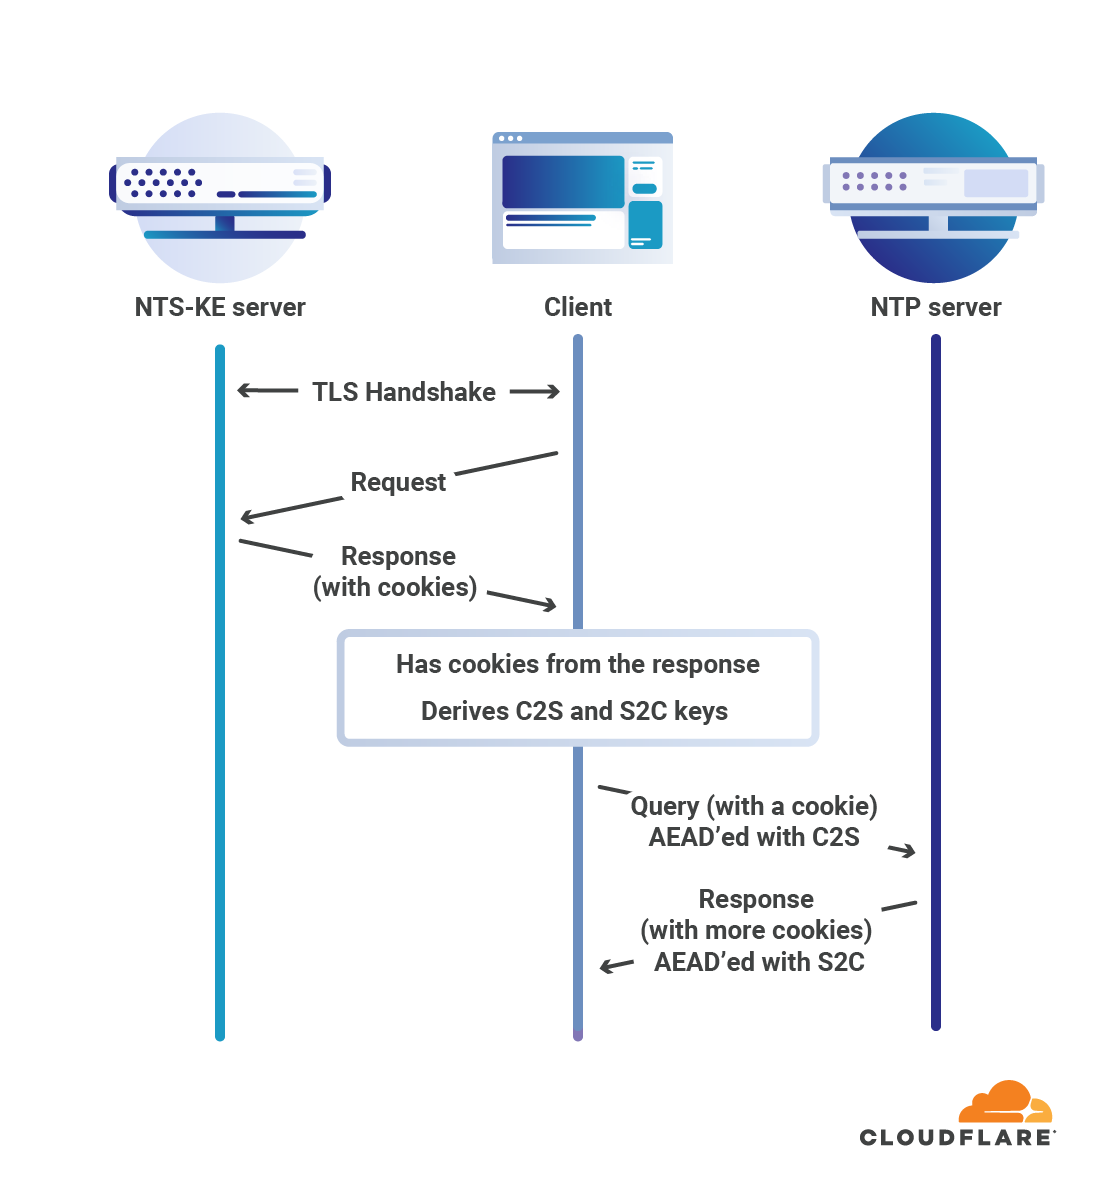
\includegraphics[height=10cm]{gorseller/cloudflare-nts.png}
\end{center}

NTS aslında yukarıda gözüktüğü gibi iki alt-protokolden oluşuyor. İlk
Cloudflare'in geliştirdiği güvenlik katmanı olan Network Time Security Key
Exchange (görselde "NTS-KE server" olarak geçiyor); ikincisi ise her
bilgisayarın kullandığı bildiğimiz Network Time Protocol (NTP) servisinin son
sürümü. Güvenli tarih/saat işlemleri yapmak için artık ilk NTS-KE ile konuşup
bazı anahtarları alıp sonra NTP sunucusu ile konuşarak güncel tarih ve zaman
bilgisini edineceğiz. Şöyle ki:
\begin{enumerate}
\item İlk aşamada NTS-KE ile şu işlemler yapılır:
\begin{enumerate}
\item Öncelikle NTS-KE sunucu ile TLS üzerinden güvenli bir iletişim kuruluyor.
(Burası bildiğimiz HTTPS)
\item İkinci aşamada kullanılacak AEAD algoritmasına karar verilir.
\item İkinci protokole karar verilir. Şu an sadece NTPv4 ile nasıl alışacağı
tanımlanmış.
\item Tarih/saat bilgilerinin alınacağı NTP sunucusunun IP adresi ve portu
belirlenir.
\item İkinci aşamada kullanmak için çerezler oluşturulur.
\item TLS oturumunda iki simetrik anahtar (C2S ve S2C) oluşturulur.
\end{enumerate}
\item İkinci aşamada ise NTP sunucusu ile:
\begin{enumerate}
\item İstemci, NTS-KE tarafından verilen anahtarı (C2S) ve çerezleri
kullanarak NTP sunucusuna tarih/saat bilgisi isteği gönderir.
\item NTP sunucusu da yine bir anahtar ile (S2C) kullanıcıya güncel
tarih/saat bilgilerini ve saklaması gereken yeni çerezleri güvenli bir
şekilde ulaştırır.
\end{enumerate}
\end{enumerate}
Birinci aşama tamamlandıktan sonra artık ikinci aşama sürekli yeni güvenlik
çerezlerini ileterek tekrarlanabilir. Tarih/saat sunucuları özellikle para
transferi gibi kritik işlerde çok büyük öneme sahip, bu yüzden de bu katmanın
güvenliği çok önemli. Bahsetmeden geçmek istemedim.
\section{Mozilla, klasörden eklenti yükleme \href{https://www.zdnet.com/article/mozilla-to-stop-supporting-sideloaded-extensions-in-firefox/}{seçeneğini kaldırmaya hazırlanıyor}}
\label{sec:org2db9bd4}
Firefox ve birçok modern tarayıcıda eklenti desteği artık olmazsa olmazlardan.
Bu eklentiler tarayıcıların kendi market sistemleri dışında eklentinin
sıkıştırılmış halini indirip onu tarayıcının kurulu olduğu dizindeki bir
klasöre atarak da kurulabiliyor fakat Mozilla, Firefox tarayıcısından bu
özelliği kaldırmayı planlıyor. Bu hafta yayınladıkları \href{https://blog.mozilla.org/addons/2019/10/31/firefox-to-discontinue-sideloaded-extensions/}{blog yazısında} sürecin
nasıl işleyeceğini açıklamış.

11 Şubat 2020 ayında yayınlanması planan Firefox 73 sürümünde de ilgili
klasördeki eklentiler okunacak fakat bunlar kopyalanarak kullanıcıya
gösterilerek normal eklenti gibi kurulacak. 10 Mart 2020 tarihinde
yayınlanması planan Firefox 74 sürümünde ise bu destek tamamen kaldırılacak.
Bu desteğin kaldırılmasının sebebi olarak ise güvenlik gösterilmiş, ilgili
klasöre gönderilen zararlı bir eklenti de firefox'a kurulabildiği için
tehlikeli bir durum oluşuyordu. Elbette sadece zararlı eklentiler gönderilmek
için kullanılmıyordu, bazı tarayıcı entegrasyonu gerektiren uygulamalar da bu
şekilde kuruyordu kendini firefox'a ama maalesef kurunun yanında yaş da
yanıyor.

Bu haberin biz geliştiricileri ilgili kısmı ise şöyle, biliyorsunuz bizler
eklenti geliştirirken kendi bilgisayarımızdaki sürekli deneyerek ilerliyoruz
dolayısıyla markette yayınlamadan eklentiyi kendi bilgisayarımızdaki Firefox'a
yükleyebilmemiz gerekiyor. Bu durumda elimizdeki bir seçenek gitti fakat
burada yanlış anlaşılma oluşmasın biz hala daha bilgisayarımızdaki bir XPI
dosyasını seçerek onu eklenti olarak kurabileceğiz, kaldırılan özelliği iyi
anlamak gerek.
\section{Yaklaşan Etkinlikler}
\label{sec:org29d65f2}
\begin{longtable}{|p{8cm}|l|l|}
\hline
Etkinlik İsmi & Yeri & Tarihi\\
\hline
\endfirsthead
\multicolumn{3}{l}{Önceki sayfadan devam ediyor} \\
\hline

Etkinlik İsmi & Yeri & Tarihi \\

\hline
\endhead
\hline\multicolumn{3}{r}{Devamı sonraki sayfada} \\
\endfoot
\endlastfoot
\hline
\href{https://www.eventbrite.com/e/arduino-ile-robotik-programlama-tickets-79692176445}{Arduino ile Robotik Programlama: Atölye ve Uygulama} & Antalya & 5 Kasım 19:00\\
\href{https://www.eventbrite.com/e/siber-farkndalk-ve-kullanc-guvenligi-tickets-78765488697}{Siber Farkındalık ve Kullanıcı Güvenliği} & İstanbul & 6 Kasım 14:00\\
\href{https://kommunity.com/software-craftsmanship-turkey/events/sosyal-ve-teknik-yonleri-ile-acik-kaynaga-nasil-katki-yapabiliriz}{Sosyal ve Teknik Yönleri ile: Açık Kaynağa Nasıl Katkı Yapabiliriz?} & İstanbul & 6 Kasım 19:00\\
\href{https://www.eventbrite.com/e/devops-tickets-78249134267}{DevOps} & İstanbul & 7 Kasım 19:00\\
\hline
\end{longtable}
\section{Diğer Haberler}
\label{sec:org06fa95e}
\begin{itemize}
\item ProtonMail, iOS uygulamasını \href{https://protonmail.com/blog/ios-open-source/}{açık kaynak yaptı}. \href{https://github.com/ProtonMail/ios-mail}{GitHub Deposu}
\item TimescaleDB, yeni \href{https://blog.timescale.com/blog/building-columnar-compression-in-a-row-oriented-database/}{sıkıştırma kabiliyetlerini duyurdu}.
\item Microsoft, OpenJDK projesine \href{https://mail.openjdk.java.net/pipermail/discuss/2019-October/005173.html}{katkı yapmaya hazırız dedi}.
\item Repl.it, kendi sistemleri için geliştirdiği paket yöneticisini \href{https://repl.it/site/blog/upm}{açık kaynak
yaptı}: \href{https://github.com/replit/upm}{upm (Universal Package Manager)}
\item Rust ana geliştirici takımından geliştiricilere çağrı: \href{https://blog.rust-lang.org/2019/10/29/A-call-for-blogs-2020.html}{2020 yılında Rust'dan
beklentileriniz neler?}
\item Python, \href{https://docs.python.org/3.5/whatsnew/changelog.html\#python-3-5-8}{3.5.8 sürümü duyuruldu}.
\item JDK 14 için \href{https://mail.openjdk.java.net/pipermail/jdk-dev/2019-October/003517.html}{çalışmalar başladı}.
\item Android Studio \href{https://androidstudio.googleblog.com/2019/10/android-studio-36-beta-2-available.html?m=1}{3.6 Beta 2 sürümü duyuruldu}.
\item Swift takımı, \href{https://swift.org/server/}{Swift Server Çalışma Grubu} ile ilgili \href{https://swift.org/blog/sswg-update/}{yıllık rapor yayınladı}.
\item Go programlama dilinin 1.13.4 ve 1.12.13 \href{https://groups.google.com/forum/m/\#!topic/golang-nuts/rkSaxR1oz0c}{sürümleri duyuruldu}. \href{https://golang.org/doc/devel/release.html\#go1.13.minor}{Değişiklik
Notları}
\item Babylon takımı, Health uygulamalarında kullandıkları Kotlin için yazılmış
\href{https://medium.com/babylon-engineering/introducing-orbit-mvi-for-kotlin-and-android-62491f4e3234}{kütüphaneyi açık kaynak yaptı}: \href{https://github.com/babylonhealth/orbit-mvi}{Orbit MVI}.
\item OpenAPI Generator, \href{https://github.com/OpenAPITools/openapi-generator/releases/tag/v4.2.0}{v4.2.0 sürümünü duyurdu}.
\item Microsoft, platformlar-arası dağıtık uygulama geliştirme kütüphanesi
\href{https://github.com/dotnet/orleans}{Orleans}'in \href{https://devblogs.microsoft.com/dotnet/orleans-3-0/}{3.0 sürümünü duyurdu}.
\item Ruby kod kalitesi raporlama aracı RubyCritic, \href{https://www.fastruby.io/blog/code-quality/code-coverage/rubycritic-4-2-0-simplecov-support.html}{v4.2.0 sürümünü yayınlandı}.
\item Rust ile yazılmış yazı arama ve indeksleme sunucusu \href{https://github.com/mosuka/bayard}{Bayard}, ilk sürümü
\href{https://github.com/mosuka/bayard/releases/tag/v0.1.0}{0.1.0'ı duyurdu}.
\item Alternatif Rust derleyicisi mrustrc, \href{https://github.com/thepowersgang/mrustc/releases/tag/v0.9}{v0.9 sürümü çıkardı}.
\item Tide, Rust web sunucusu \href{https://github.com/http-rs/tide/releases/tag/0.3.0}{0.3.0 sürümünü duyurdu}.
\item Lazarus \href{https://forum.lazarus.freepascal.org/index.php/topic,47269.0.html}{2.0.6 çıktı}.
\item Immer \href{https://github.com/immerjs/immer}{v5.0.0 çıktı}.
\end{itemize}
\section{Lisans}
\label{sec:org96dcc63}
\begin{center}
\begin{center}

\includegraphics[height=1.5cm]{../../../img/CC_BY-NC-SA_4.0.png}
\end{center}

\href{yazilim-gundemi-16.pdf}{Yazılım Gündemi - 16} yazısı \href{https://erenhatirnaz.github.io}{Eren Hatırnaz} tarafından \href{http://creativecommons.org/licenses/by-nc-sa/4.0/}{Creative Commons
Atıf-GayriTicari-AynıLisanslaPaylaş 4.0 Uluslararası Lisansı} (CC BY-NC-SA 4.0)
ile lisanslanmıştır.
\end{center}
\end{document}
